\documentclass[conference]{IEEEtran}
\usepackage{amsmath,amssymb,amsthm,mathtools,booktabs,cite,tikz,graphicx,url}
\usetikzlibrary{arrows.meta}
\newtheorem{lemma}{Lemma}
\newtheorem{proposition}{Proposition}
\newtheorem{theorem}{Theorem}
\newtheorem{corollary}{Corollary}
\newcommand{\E}{\mathcal{E}}
\newcommand{\Hn}{\mathcal{H}}
\newcommand{\B}{\mathcal{B}}
\newcommand{\Pc}{\mathrm{PC}}
\newcommand{\Cc}{\mathrm{CC}}
\newcommand{\Val}{\mathrm{Valid}}
\newcommand{\Sel}{\mathrm{Sel}}
\newcommand{\Cm}{\mathrm{Committed}}
\newcommand{\W}{\mathcal{W}}
\newcommand{\Av}{\mathrm{Av}}
\newcommand{\words}[1]{\par\noindent\textit{In words.} #1\par\smallskip}
\begin{document}
\title{Witnessed Policy: Quorum-Committed, Edge-Validated Policy for SD-WAN}
\author{\IEEEauthorblockN{Blessing Honmane}
\IEEEauthorblockA{SafeLinx Technology\\blessing.honmane@safelinx.ng}}
\maketitle

\begin{abstract}
An SD-WAN controller is a single point of policy authority. We keep it trusted for availability only: policy is a signed hash chain validated at every edge (layer~1), and a two-phase quorum commit with administrator-started round change makes the chain fork-free at enforcement (layer~2). With $n$ edges, at most $b$ Byzantine and $c$ further offline, quorum $T=\lceil (n+b+1)/2\rceil$ is safe and live iff $n\ge 3b+2c+1$, so each offline edge costs two extra edges instead of three. We prove unique commit, show that one-phase commit with claim-based recovery is unsafe, bound revocation, and check the core with TLA$^+$/TLC (safety, liveness, trace validation) and a prototype of real edge processes with WireGuard and nftables, against baselines and a 30-record incident corpus.
\end{abstract}

\section{Introduction}
A stolen controller credential should not be able to rewrite a network's policy, and tolerating offline branches should not require extra sites. Witnessed Policy meets both: the controller is untrusted for safety, and the quorum is sized by separating Byzantine edges ($b$) from offline ones ($c$). The consequence is that $n\ge3b+2c+1$ edges suffice instead of $3(b{+}c)+1$. For $n{=}12$ edges, one compromised and four offline ($b{=}1,c{=}4$), the quorum is $T{=}7$ and a commit is possible with probability
\begin{equation}\label{eq:avail}
\Av(n,b,Q,a)=\sum_{k=Q}^{n-b}\binom{n-b}{k}a^k(1-a)^{n-b-k}
\end{equation}
($Q$ the quorum, $a$ per-edge availability, Byzantine edges silent), whereas treating offline edges as Byzantine would need $n\ge16$ and, at $n{=}12$, lowers availability from $0.997$ to $0.910$ at $a{=}0.9$ (Table~\ref{tab:avail}).
\begin{table}[b]
\centering\caption{Commit availability, eq.~\eqref{eq:avail}: separated quorum $T(n,b)$ vs.\ simple $T(n,b{+}c)$.}\label{tab:avail}
\begin{tabular}{@{}lcccc@{}}
\toprule
$(n,b,c)$ & $a$ & $T_{sep}$ & $\Av_{sep}$ & $\Av_{simple}$\\
\midrule
(12,1,4)& 0.90 & 7 & 0.9972 & 0.9104\\
(12,1,4)& 0.95 & 7 & 0.9999 & 0.9848\\
(16,1,4)& 0.90 & 9 & 0.9997 & 0.9873\\
(20,2,6)& 0.90 & 12 & 0.9988 & 0.9018\\
\bottomrule
\end{tabular}
\end{table}

\begin{figure}[t]\centering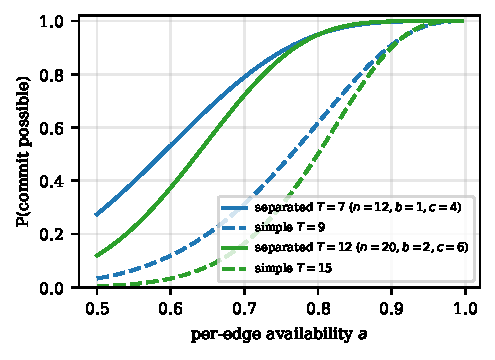
\includegraphics[width=\columnwidth]{fig/fig_avail}\caption{Commit availability vs.\ per-edge availability, separated vs.\ simple quorum.}\label{fig:avail}\end{figure}
\textbf{Positioning.} We do not propose a new Byzantine agreement protocol. The quorum arithmetic is UpRight's~\cite{upright}, the round change follows PBFT~\cite{pbft}, and the per-round prepare lock follows FastPay~\cite{fastpay}. What is new is their use for SD-WAN policy enforcement: edges validate each entry against the policy rules (tiered approvals, protected invariants), decide each slot themselves and enforce only committed entries, so a compromised controller cannot forge or fork policy. We also bound revocation and freshness for the resulting data plane and measure its cost with real WireGuard and nftables enforcement.

\textbf{Contributions.}
(1) Unique commit under $\le b$ Byzantine edges, across rounds and epochs (Thm.~\ref{thm:unique}).
(2) The mixed bound for this protocol (Prop.~\ref{prop:tight}), safe iff $Q\ge T$ and live iff $Q\le n{-}b{-}c$, and a proof that one-phase commit with claim-based recovery is unsafe (Prop.~\ref{prop:onephase}).
(3) Lost-record accounting and an observer rule (Prop.~\ref{prop:lost}).
(4) Certified time and revocation bounds (Props.~\ref{prop:time},~\ref{prop:revoke}).
(5) TLC safety, liveness and trace-validation checks; baselines S0 and S3; an attack-model simulation, an outage simulation and a 30-record incident corpus; and a prototype whose edges are real processes with WireGuard tunnels and nftables enforcement (Sections~\ref{sec:tlc},~\ref{sec:eval}).
Motivation: controller compromise is a recurring SD-WAN threat~\cite{gordeychik,ambusher,cso}.

\textbf{Not claimed.} The node bound is UpRight's $2u{+}r{+}1$ with $u{=}b{+}c$, $r{=}b$; collusion of $\ge m$ administrators is out of scope. \textbf{Scope.} The paper offers a design, proofs, model checking and a single-host prototype. The incident corpus was coded by two coders ($\kappa{=}1.00$). A multi-host deployment is future work. \textbf{Artifact.} Code, specifications, traces and the incident corpus are at \url{https://github.com/honbles/Witnessed-Policy}.

\section{Mechanism in One Page}
\textbf{Intuition.} Edges, not the controller, decide each policy slot. An edge \emph{prepares} at most once per round; $T$ prepares form a \emph{prepared certificate} (PC), proof that no other value can be prepared in that round. Only an edge holding a PC \emph{commits}; $T$ commits form a \emph{commit certificate} (CC), and edges enforce an entry only with a CC. If proposals split, no PC forms and the slot is stuck. One administrator then starts a \emph{round change}: edges promise to ignore lower rounds and report the highest PC they hold, and the new round must adopt the value of the highest reported PC. A value that may already have committed is therefore never abandoned, because any $T$ reports overlap the $T$ committers in an honest edge (Fig.~\ref{fig:flow}).

\begin{figure*}[t]
\centering
\resizebox{0.92\textwidth}{!}{%
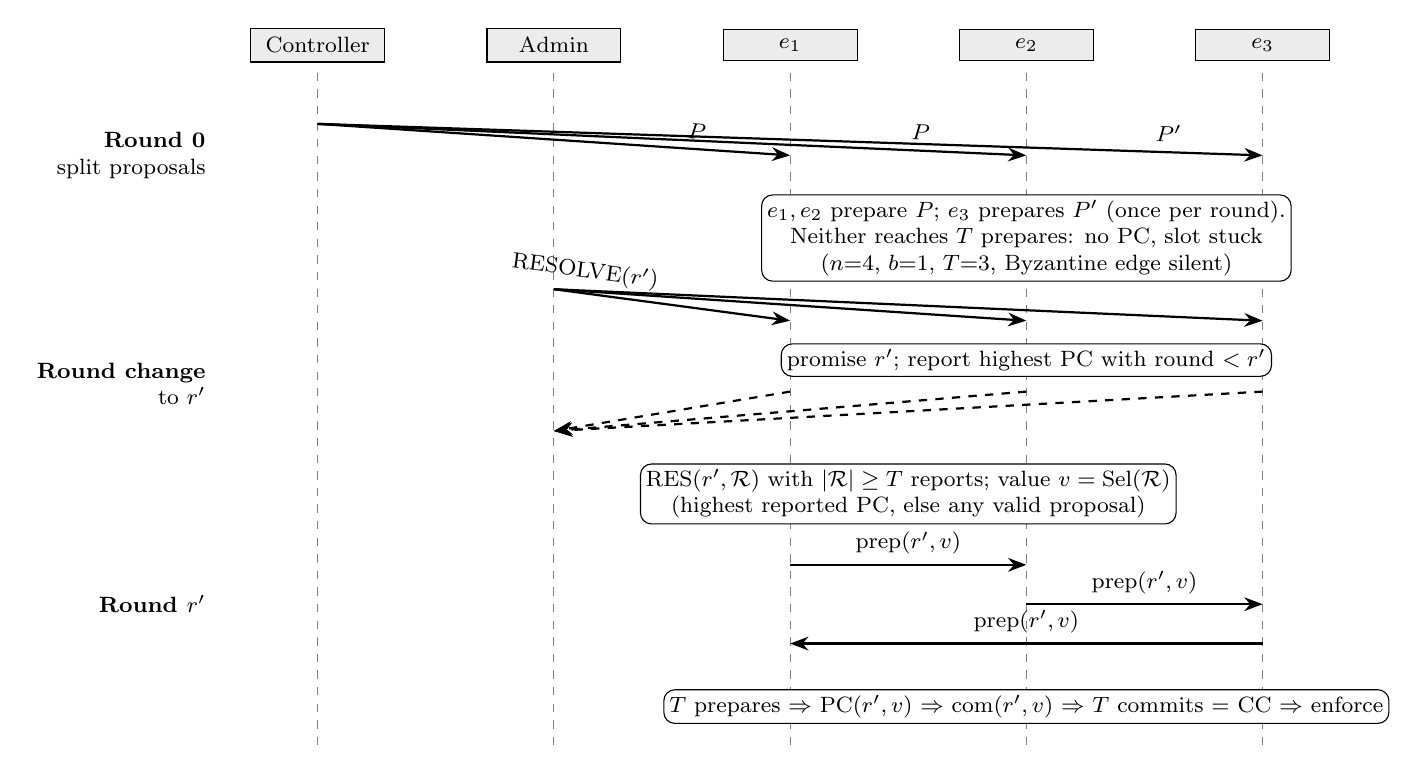
\begin{tikzpicture}[x=1cm,y=1cm,>=Stealth,font=\footnotesize,
 life/.style={dashed,gray},msg/.style={->,thick},rep/.style={->,thick,dashed},
 note/.style={draw,rounded corners,fill=white,inner sep=2pt,align=center}]
\foreach \x/\n in {0/Controller,3/Admin,6/$e_1$,9/$e_2$,12/$e_3$}{
 \node[draw,fill=gray!15,minimum width=1.7cm] at (\x,0) {\n};
 \draw[life] (\x,-0.35)--(\x,-8.9);}
\node[anchor=east,align=right] at (-1.3,-1.4) {\textbf{Round 0}\\split proposals};
\node[anchor=east,align=right] at (-1.3,-4.3) {\textbf{Round change}\\to $r'$};
\node[anchor=east,align=right] at (-1.3,-7.1) {\textbf{Round $r'$}};
\draw[msg](0,-1)--(6,-1.4) node[pos=.8,above,sloped]{$P$};
\draw[msg](0,-1)--(9,-1.4) node[pos=.85,above,sloped]{$P$};
\draw[msg](0,-1)--(12,-1.4) node[pos=.9,above,sloped]{$P'$};
\node[note] at (9,-2.45) {$e_1,e_2$ prepare $P$; $e_3$ prepares $P'$ (once per round).\\ Neither reaches $T$ prepares: no PC, slot stuck\\($n{=}4$, $b{=}1$, $T{=}3$, Byzantine edge silent)};
\draw[msg](3,-3.1)--(6,-3.5) node[pos=.12,above,sloped]{RESOLVE$(r')$};
\draw[msg](3,-3.1)--(9,-3.5);
\draw[msg](3,-3.1)--(12,-3.5);
\draw[rep](6,-4.4)--(3,-4.9);
\draw[rep](9,-4.4)--(3,-4.9);
\draw[rep](12,-4.4)--(3,-4.9);
\node[note] at (9,-4.0) {promise $r'$; report highest PC with round $<r'$};
\node[note] at (7.5,-5.7) {RES$(r',\mathcal R)$ with $|\mathcal R|\ge T$ reports; value $v=\Sel(\mathcal R)$\\(highest reported PC, else any valid proposal)};
\draw[msg](6,-6.6)--(9,-6.6) node[midway,above]{prep$(r',v)$};
\draw[msg](9,-7.1)--(12,-7.1) node[midway,above]{prep$(r',v)$};
\draw[msg](12,-7.6)--(6,-7.6) node[midway,above]{prep$(r',v)$};
\node[note] at (9,-8.4) {$T$ prepares $\Rightarrow$ PC$(r',v)$ $\Rightarrow$ com$(r',v)$ $\Rightarrow$ $T$ commits $=$ CC $\Rightarrow$ enforce};
\end{tikzpicture}}
\caption{Message flow for $n{=}4,b{=}1,T{=}3$ with the Byzantine edge silent (an active one could complete a PC for $P$): a split round 0 is stuck; an administrator starts round $r'$; the value is forced by the highest reported PC, then prepare$\to$commit as usual.}\label{fig:flow}
\end{figure*}

\section{Model}
\subsection{Entities, faults, chain}
Edges $\E=\{1,\dots,n\}$; Byzantine $\B\subseteq\E$, $|\B|\le b$; offline $C\subseteq\E\setminus\B$, $|C|\le c$; honest $\Hn=\E\setminus\B$; up $U=\E\setminus(\B\cup C)$. Administrators $\mathcal A$; entry tier $\theta(\eta)\in\{\mathsf{L0},\mathsf{L1},\mathsf{L2},\mathsf{L3},\mathsf{R}\}$ with threshold $m_\theta$. Honest clocks differ by at most $\sigma$.
\begin{equation}\label{eq:T}
T=\Big\lceil \tfrac{n+b+1}{2}\Big\rceil .
\end{equation}
Entry $\eta_s=(s,h_{s-1},op,\theta,\mathsf{Ap})$, $h_s=\mathrm{hash}(\eta_s)$, $\mathsf{Ap}$ the approvals. State $S_s=\mathrm{apply}(S_{s-1},\eta_s)$, $S_0$ from genesis $G_0$. $\mathrm{WF}(S)$ says the state is well formed, $\mathrm{Prot}(S)$ that no grant in $S$ crosses a protected pair, $\Gamma(S)$ is the set of grants in $S$, $\mathrm{Tr}(f)$ the transit sites of a flow $f$, and $\mathrm{inst}_u(\gamma)$ that site $u$ has installed grant $\gamma$.
\begin{align}
\mathrm{Auth}(\eta)&\Leftrightarrow \big|\{\alpha\in\mathcal A:\mathrm{vrf}_\alpha(\eta)\}\big|\ge m_{\theta(\eta)},\\
\Val(S,\eta)&\Leftrightarrow \mathrm{Auth}(\eta)\wedge \mathrm{WF}(S')\wedge \mathrm{Prot}(S'),\nonumber\\
&\qquad S'=\mathrm{apply}(S,\eta).
\end{align}
$\Val$ is a deterministic function of the shared prefix. The protected set $\Pi(S')=\Pi(S)$ unless $op$ removes an invariant at tier $\mathsf{L3}$.

\subsection{Attestations, certificates, rules}
For slot $s$, round $r$, digest $v$: $P_{s,r}(v)$, $K_{s,r}(v)\subseteq\E$ are the edges that issued $\langle\mathrm{prep},s,r,v\rangle$, $\langle\mathrm{com},s,r,v\rangle$.
\begin{align}
\Pc(s,r,v)&\Leftrightarrow |P_{s,r}(v)|\ge T,\\
\Cc(s,r,v)&\Leftrightarrow |K_{s,r}(v)|\ge T,\\
\Cm(s,v)&\Leftrightarrow \exists r:\ \Cc(s,r,v).
\end{align}
Edges enforce $\eta_s$ only if $\Cm(s,\mathrm{hash}(\eta_s))$. Fix $s$. An honest edge $e$ keeps a durable promise $\pi_e$ (init $0$) and the set $\W_e$ of prepared certificates it holds. Certificates are unforgeable; Byzantine edges may sign anything; every attestation, promise and report is durable before it is sent.
\begin{description}\itemsep0pt
\item[R1] $\mathrm{prep}(r,v)$ iff $\Val(S_{s-1},v)\wedge\pi_e\le r\wedge$ no prior prepare of $e$ in round $r$ $\wedge\,(r{=}0\vee(r,v)\in\mathrm{Res})$; then $\pi_e\leftarrow r$.
\item[R2] $\mathrm{com}(r,v)$ iff $(r,v)\in\W_e\wedge\pi_e\le r\wedge$ no prior commit of $e$ in round $r$.
\item[R3] $\mathrm{promise}(r')$ iff $r'>\pi_e$; then $\pi_e\leftarrow r'$ and $e$ reports $\rho_e(r')=\max_{\mathrm{round}}\{(r,v)\in\W_e:r<r'\}$ or $\bot$.
\item[R4] $(r',v)\in\mathrm{Res}$ iff an admin-signed $\mathrm{RES}(r',\mathcal R)$ carries $|\mathcal R|\ge T$ edge-signed reports bound to $r'$, each holding only certificates of round $<r'$, and $v\in\Sel(\mathcal R)$.
\item[A5] An edge attests at slot $s$ only if it holds $\eta_1..\eta_{s-1}$ with certificates.
\end{description}
\begin{equation}
\Sel(\mathcal R)=\begin{cases}\{v^\star\}&\text{if a certificate is carried}\\[-1pt]&(v^\star\text{ of the max round})\\ \text{any valid }v&\text{otherwise.}\end{cases}
\end{equation}

\section{Safety}
\begin{lemma}[intersection]\label{lem:int}
$|Q_1|,|Q_2|\ge T\Rightarrow |Q_1\cap Q_2|\ge 2T-n\ge b+1$, so $(Q_1\cap Q_2)\setminus\B\ne\emptyset$.
\end{lemma}
\begin{proof}
$|Q_1\cap Q_2|\ge |Q_1|+|Q_2|-n$ and $2T\ge n+b+1$.
\end{proof}
\begin{lemma}[one prepared value per round]\label{lem:one}
$\Pc(r,v)\wedge\Pc(r,w)\Rightarrow v=w$.
\end{lemma}
\begin{proof}
By Lemma~\ref{lem:int} some honest $e\in P_r(v)\cap P_r(w)$; R1 allows one prepare per round.
\end{proof}
\begin{lemma}[commit implies prepared]\label{lem:cp}
$\Cc(r,v)\Rightarrow \Pc(r,v)\wedge \Val(S_{s-1},v)$.
\end{lemma}
\begin{proof}
(1) $|K_r(v)|\ge T>b$, so $K_r(v)$ contains an honest edge $e$. (2) By R2, $e$ issued $\langle\mathrm{com},s,r,v\rangle$ only after holding a prepared certificate for $(r,v)$, that is, $T$ signed prepares for $v$ in round $r$. Certificates are unforgeable, so $|P_{s,r}(v)|\ge T$ and $\Pc(r,v)$ holds. (3) At most $b$ of these prepares are Byzantine, so at least $T-b\ge1$ come from honest edges. By R1 each prepared $v$ only after $\Val$ held on its prefix, and that prefix is the unique $S_{s-1}$ (A5 and the induction on slots in Thm.~\ref{thm:unique}). Hence $\Val(S_{s-1},v)$.
\end{proof}
\words{No two different entries are ever enforced for the same slot, whatever the controller does, provided at most $b$ edges are Byzantine.}
\begin{theorem}[unique commit]\label{thm:unique}
If $|\B|\le b$ and honest edges obey R1--R4 with durable records, then $\forall s:\ |\{v:\Cm(s,v)\}|\le 1$.
\end{theorem}
\begin{proof}
We argue for slot $s$ by induction on $s$: slots below $s$ have a unique committed entry, so every honest edge that attests at $s$ (A5) holds the same prefix and $\Val$ is the same predicate at all of them.

\emph{Claim} $\mathcal I(\rho,v)$: $\Cc(\rho,v)\Rightarrow\forall r\ge\rho,\ \forall w:\ \Pc(r,w)\Rightarrow w=v$. Induct on $r$.

\emph{Base} $r=\rho$. Lemma~\ref{lem:cp} gives $\Pc(\rho,v)$ and Lemma~\ref{lem:one} gives $w=v$.

\emph{Step} $r>\rho$. Let $\Pc(r,w)$ and assume $\mathcal I(\rho,v)$ for the rounds in $[\rho,r-1]$.
(1) At least one honest edge prepared $w$ in round $r$, since $T>b$. As $r>0$, R1 gives $(r,w)\in\mathrm{Res}$, so some admin-signed $\mathrm{RES}(r,\mathcal R)$ has $|\mathcal R|\ge T$ and $w\in\Sel(\mathcal R)$.
(2) Let $K=K_\rho(v)$. By Lemma~\ref{lem:int} some honest $e^\star$ lies in $\mathcal R\cap K$.
(3) $e^\star$ committed in round $\rho$ \emph{before} it reported: its report sets $\pi_{e^\star}\ge r>\rho$ (R3), and R2 requires $\pi\le\rho$ to commit in round $\rho$.
(4) By R2, $e^\star$ then held a prepared certificate for $(\rho,v)$. Certificate sets only grow, so its report carries a certificate of some round in $[\rho,r-1]$, the highest it holds below $r$.
(5) Every certificate in $\mathcal R$ has round $<r$. By $\mathcal I$ on $[\rho,r-1]$, each one of round $\ge\rho$ is for $v$, whoever reported it, because certificates cannot be forged. By (4) the maximum-round certificate in $\mathcal R$ has round $\ge\rho$, and certificates of one round carry one value (Lemma~\ref{lem:one}). So $\Sel(\mathcal R)=\{v\}$ and $w=v$.

\emph{Conclusion.} If $\Cm(s,v)$ and $\Cm(s,w)$, say $\Cc(\rho_v,v)$ and $\Cc(\rho_w,w)$ with $\rho_v\le\rho_w$, then $\Pc(\rho_w,w)$ by Lemma~\ref{lem:cp}, hence $w=v$ by $\mathcal I(\rho_v,v)$.
\end{proof}
\words{Edges never disagree about history, and every enforced entry carries the approvals its tier requires and respects the protected invariants. A forged controller entry is never enforced.}
\begin{corollary}[no fork; authorization; invariants]\label{cor:fork}
(a) For honest $e,e'$, $\mathrm{enf}_e(s)=v$ and $\mathrm{enf}_{e'}(s)=v'$ imply $v=v'$, so enforced histories are prefix-comparable. (b) $\forall s:\ \mathrm{Auth}(\eta_s)\wedge\mathrm{Prot}(S_s)$ and $\Pi(S_s)\supseteq\Pi(S_0)$ minus $\mathsf{L3}$-removed elements; an entry with $|\mathsf{Ap}|<m_\theta$ is never committed.
\end{corollary}
\begin{proof}
(a) Enforcement needs a CC; apply Thm.~\ref{thm:unique}. (b) Lemma~\ref{lem:cp} and induction on $s$ (unique $S_{s-1}$). A forged entry fails $\mathrm{Auth}$, so only $\le b<T$ edges attest.
\end{proof}
\words{Membership changes cannot open a window for two histories.}
\begin{proposition}[epochs]\label{prop:epoch}
Membership $M_s$ is a function of $S_{s-1}$; ENROLL/EVICT in $\eta_s$ act from $s{+}1$; attestations of other epochs are ignored. If $|\B\cap M_s|\le b_s$ with $T_s=T(|M_s|,b_s)$ for all $s$, Thm.~\ref{thm:unique} holds for all $s$.
\end{proposition}
\begin{proof}
Induction on $s$: $S_{s-1}$ unique $\Rightarrow M_s$ unique $\Rightarrow$ slot $s$ is an instance of Thm.~\ref{thm:unique} with $(M_s,T_s)$.
\end{proof}
\words{$T$ is the smallest safe quorum, and $n{-}b{-}c$ is the largest quorum that is still reachable when $c$ edges are offline; a feasible quorum exists exactly when $n\ge3b+2c+1$.}
\begin{proposition}[tightness]\label{prop:tight}
For quorum $Q$: (a) safety against all $|\B|\le b$ iff $Q\ge T$; (b) liveness with $\B$ silent and $|C|=c$ iff $Q\le n-b-c$. Hence a feasible $Q$ exists iff
\begin{equation}\label{eq:bound}
n\ge 3b+2c+1,
\end{equation}
versus $n\ge 3(b+c)+1$ if offline edges are treated as Byzantine.
\end{proposition}
\begin{proof}
(a) ``If'' is Thm.~\ref{thm:unique}. If $Q<T$ then $2Q-n\le b$; choose $Q_1,Q_2$ with $|Q_1\cap Q_2|\le b$ and let $\B\supseteq Q_1\cap Q_2$ sign both $v\ne w$: two certificates. (b) A commit needs $Q$ attestations from $U$. Combine: $\lceil\frac{n+b+1}{2}\rceil\le n-b-c\iff n\ge3b+2c+1$ (RHS integer).
\end{proof}
\noindent Example: $n{=}12,b{=}1,c{=}4$ gives $T{=}7=n-b-c$; the simple rule needs $n\ge16$.
\begin{figure}[t]\centering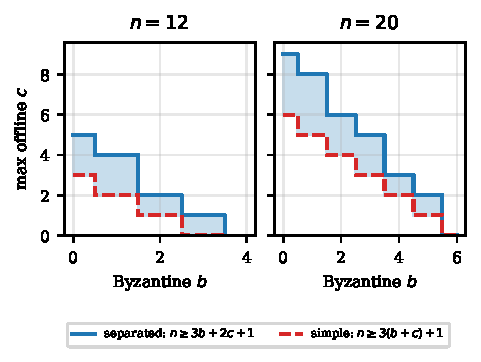
\includegraphics[width=\columnwidth]{fig/fig_region}\caption{Tolerable $(b,c)$: separated (solid) vs.\ simple (dashed); shaded gain.}\label{fig:region}\end{figure}
\words{One-phase commit whose recovery relies on uncertified reports cannot be repaired by enlarging the quorum: such reports can be forged. Faster one-phase protocols exist at larger $n$, for example FaB~\cite{fab} with $n\ge5b+1$.}
\begin{proposition}[claim-based one-phase commit is unsafe]\label{prop:onephase}
Let commit need $Q\in[T,n-b-c]$ attestations and RES select the value of the highest-round \emph{claimed} last attestation (no certificates). For every $n$ and $b\ge1$ there is a run with two committed values.
\end{proposition}
\begin{proof}
Round 0: take $K$ with $|K|=Q$, $z\in K\cap\B$, $K\setminus\{z\}\subseteq U$ (possible since $Q-1\le n-b-c$); $K$ attests $v$, so $v$ commits. $\mathrm{RES}(2,\mathcal R)$, $|\mathcal R|=Q$, $z\in\mathcal R$: honest members report $(0,v)$ or $\bot$; $z$ reports the forged $(1,w)$. The highest claim is $(1,w)$, so $w$ is selected. In round 2 the $n-b-c\ge Q$ up honest edges all attest $w$ (R1: $\pi\le2$, $(2,w)\in\mathrm{Res}$, locking is per round), so $w$ commits without any Byzantine help. (With $\B$ the margin is $n-c\ge Q+b$.)
\end{proof}
\noindent TLC finds the same double commit for $n{=}4,5$ with $b{=}1$, and under a ``$b{+}1$ matching claims'' rule for $n{=}4,5,6$ (Table~\ref{tab:tlc}); that rule fails on ties between honest and Byzantine-supported claims. Prepared certificates remove the dependence on claims.
\words{An edge that forgets what it attested must be counted among the Byzantine ones, unless it sits out until the chain has moved past that slot.}
\begin{proposition}[lost attestation record]\label{prop:lost}
Let $L\subseteq\Hn$ lose records (and may re-attest).
(i) Thm.~\ref{thm:unique} holds with $b$ replaced by $b'\ge|\B|+|L|$ and $T=T(n,b')$.
(ii) If $T=T(n,b)$, $|\B|+|L|=b+1$ and $n+b$ is odd, unique commit can fail.
(iii) Observer rule: $\ell\in L$ with persisted head $h_\ell$ (heads are persisted before any attestation above them) attests only at slots $\ge h_\ell+2$. Then $\ell$ never double-attests; it counts in $c$, not $b$, and the bound becomes $n\ge 3b+2(c+|L|)+1$.
\end{proposition}
\begin{proof}
(i) The proof of Thm.~\ref{thm:unique} uses only that $\le b'$ edges violate R1--R3. (ii) $2T-n=b+1$ when $n+b$ is odd; take $\B\cup L$ as the overlap (TLC: $n{=}4,b{=}1$). (iii) By A5, pre-loss attestations are at slots $\le h_\ell+1$.
\end{proof}
\words{Without layer~2, a stolen key plus a partitioning controller makes edges enforce different policies; with layer~2 this never happens.}
\begin{proposition}[layer 1 alone forks]\label{prop:s1}
Under layer~1 only, with $m_\theta=1$ and one stolen key, the controller can sign $\eta\ne\eta'$ on one base and partition $\E=\E_1\sqcup\E_2$. The divergence
\begin{equation}
D(t)=\big|\{(e,e'):\mathrm{enf}_e(s)\ne\mathrm{enf}_{e'}(s)\}\big|=|\E_1||\E_2|
\end{equation}
holds until the first cross-side head arrives, unbounded under a persistent partition. Under layer~2, $D\equiv0$ (Cor.~\ref{cor:fork}).
\end{proposition}
\begin{proof}
With $m_\theta=1$ both entries satisfy $\mathrm{Auth}$; $\Val$ depends only on the shared prefix, so each side validates and enforces its entry. Layer~2 excludes this by Thm.~\ref{thm:unique}.
\end{proof}

\section{Liveness}
\words{A stuck slot always recovers when enough edges are up and one administrator is available.}
\begin{proposition}[round-change liveness]\label{prop:live}
If $n-b-c\ge T$, messages among $U$ are eventually delivered (edges retransmit issued attestations when a proposal is re-sent), and one administrator signs RES, a stuck slot commits within two rounds.
\end{proposition}
\begin{proof}
$|U|\ge T$ reports exist (R3); $\Sel$ yields a value; $U$ prepares and commits it (R1, R2).
\end{proof}

\section{Time, Freshness, Revocation}
\words{A compromised controller cannot move a certified time outside the range of honest timestamps, whose width is the honest clock skew plus the spread of their issue times.}
\begin{proposition}[certified time]\label{prop:time}
Let $k\ge T$ timestamps $t_{(1)}\le\dots\le t_{(k)}$ of a CC contain $\le b$ Byzantine ones. For $n\ge3b+1$ the median $\tilde t=t_{(\lceil k/2\rceil)}$ satisfies $\min_{\Hn}t\le\tilde t\le\max_{\Hn}t$, a range of width at most $\sigma$ plus the spread of the issue times of the honest timestamps.
\end{proposition}
\begin{proof}
$T\ge2b+1$, so $\lceil k/2\rceil\ge b+1$ and $\lfloor k/2\rfloor+1\ge b+1$: both the lowest $\lceil k/2\rceil$ and the highest $\lfloor k/2\rfloor+1$ values contain an honest one.
\end{proof}
Edges sign heads $(s,h_s,t)$ every $g$. The target slot $s^\star(t)=\max\{s:\ |\{e:\mathrm{head}_e\ge s\}|\ge b+1\}$ is committed (one honest voucher). An edge is \emph{fresh} iff it holds heads from $\ge T$ distinct edges (itself counted once) within $\Delta$ and $\mathrm{applied}_e\ge s^\star$, with $s^\star$ computed over the heads it holds. A grant is effective at $e$ before its lease expires, or later while $e$ is fresh. Requiring only $b{+}1$ heads would be unsound: a partitioned minority could vouch for itself and never learn of a revocation.
\words{A connected edge applies a revocation within about one gossip interval; an edge that is cut off stops at lease expiry.}
\begin{proposition}[revocation]\label{prop:revoke}
Let a revocation commit at $t_c$ and let $d_{\mathrm{enf}}$ be the time to remove forwarding and sessions. (a) If $e$ has delay-$\delta$ links to $\ge b+1$ honest edges, $t_{\mathrm{eff}}(e)\le t_c+4\delta+g+d_{\mathrm{enf}}$. (b) If $e$ is not fresh at any time $\ge\lambda_\gamma$, the lease expiry of the revoked grant $\gamma$ (for instance because it holds fewer than $T$ heads, being cut off from more than $n{-}T$ other edges), then $t_{\mathrm{eff}}(e)\le\lambda_\gamma+\sigma+d_{\mathrm{enf}}$.
\end{proposition}
\begin{proof}
(a) Commit attestations reach linked honest edges by $t_c{+}\delta$; their heads reach $e$ by $t_c{+}2\delta{+}g$; fetching costs $2\delta$. (b) A grant is effective at a non-fresh edge only before its lease expires, which $e$ judges with clock skew at most $\sigma$; removing forwarding and sessions then takes $d_{\mathrm{enf}}$. Freshness is a sufficient condition for staying effective beyond the lease, so no other case arises when $e$ is not fresh.
\end{proof}

\section{Enforcement and Bootstrap}
Flow $f$ is forwarded at slot $s$ iff $\exists\gamma\in\Gamma(S_s):\ f\in\gamma\wedge\forall u\in\{\mathrm{src},\mathrm{dst}\}\cup\mathrm{Tr}(f):\ \mathrm{inst}_u(\gamma)$ (two-sided, transit; default deny otherwise). Edge state $\in\{\mathrm{UNPROV},\mathrm{ANCHORED},\mathrm{SYNC},\mathrm{VERIFIED},\mathrm{VOTING}\}$ with
\begin{align}
&\mathrm{UNPROV}\to\mathrm{ANCHORED}\iff \mathrm{hash}(G_0)=h_{\mathrm{oob}},\\
&\mathrm{attest}_e(s)\Rightarrow \mathrm{st}_e=\mathrm{VOTING}\wedge s>\mathrm{head}_e,\\
&\mathrm{Fwd}_e\neq\emptyset\Rightarrow \mathrm{st}_e\ge\mathrm{VERIFIED}.
\end{align}
A substituted genesis fails the first test; such an edge is counted in $b$.

\section{Machine-Checked Results}\label{sec:tlc}
\texttt{WitnessedPolicy.tla} models one slot: honest edges explicit, Byzantine edges as maximal-power counts, durable records, promise/report/RES, offline edges, record loss. Checked: UniqueCommit, NoDoubleAttest, PreparedBeforeCommit, PromiseRespected. For three rounds ($n{=}4$) and for $n{=}7$ (two rounds) we use \texttt{WitnessedPolicyAbs.tla}, in which an edge learns certificates instantly and reports any existing lower-round certificate at least as high as its own commits; this over-approximates the explicit-knowledge model, and as a negative control it flags the violation at $T{=}2$. TLC runs with 8 workers on an 8-vCPU server and quotients by edge permutations and by swapping the two values; counts for violations are where TLC stopped. An independent Python model (edge symmetry only) reaches $145{,}708$ states; $18$ of them are invariant under the value swap, and Burnside's lemma gives $(145{,}708{+}18)/2=72{,}863$, exactly TLC's count.
\begin{table}[t]
\centering\caption{TLC results (distinct states).}\label{tab:tlc}
\scriptsize
\begin{tabular}{@{}p{3.7cm}p{2.0cm}r@{}}
\toprule
Configuration & Result & States\\
\midrule
$n{=}4,b{=}1,T{=}3$, rounds 0..1 & no violation & 72,863\\
same, rounds 0..2 (abstract) & clean, exhaustive & 6,542,584\\
$n{=}7,b{=}2,T{=}5$, rounds 0..1 (abstract) & clean, exhaustive & 1,048,806\\
lost record, $T(n,b)$, $n{=}4$ & violation & --\\
lost record, $T(n,b{+}1)=4$ & no violation & 61,983\\
lost record, observer, $T{=}3$ & no violation & 426,322\\
$n{=}6,b{=}1,c{=}1$ (bound tight) & commit reachable & 344\\
$n{=}5,b{=}1,c{=}1$; $n{=}6,b{=}1,c{=}2$ & no commit & 32; 32\\
one-phase highest, $n{=}4,5$ & double commit & 917; 5,175\\
one-phase matching, $n{=}4,5,6$ & double commit & 1,031; 7,757; 7,730\\
liveness under fairness, $n{=}4$, rounds 1; 2 & holds & 2,040; 158,458\\
liveness, $T$ above the honest edges & fails (control) & 216\\
\bottomrule
\end{tabular}
\end{table}
\textbf{Liveness.} In \texttt{WPLiveness.tla} Byzantine edges are silent, the administrator issues at most one RES value per round, and every honest action is weakly fair; $\Diamond\,\mathrm{Committed}\ne\emptyset$ holds from every initial state (rows above). A Python model agrees on recovery: every round-0 split without a certificate recovers via RES \emph{iff} $n-b-c\ge T$ ($25/25$ for $n{=}4,b{=}1,c{=}0$; $221/221$ for $n{=}6,b{=}1,c{=}1$, exactly at the bound; $0/79$ for $n{=}5,b{=}1,c{=}1$, one below it), matching Prop.~\ref{prop:tight}(b).

\textbf{Trace validation.} Prototype event logs are translated to TLA$^+$ and TLC checks that the spec's \texttt{Next} admits them step by step. All six traces are admitted: split-and-RESOLVE (T20), two conflicting RES (T21), an equivocating Byzantine edge, offline edges, and two traces from real edge processes ($n{=}16$ and $32$); a trace with a commit attestation moved before any prepare is rejected.

\textbf{Property-based fuzz.} 250 random entries (random ops, tiers, approval subsets, forged tiers, stale epochs) go through the full protocol at $n{=}7$. S2 and S1 commit 94 and reject 156, with $0$ violations of ProtectedPreserved, Auth, no-default-permit and the cipher floor, and one chain at every edge; S0 (edges trust the controller) commits all 250 with $6{,}581$ violations. The fuzz motivated one validity rule: a protected pair that existing grants already cross must fail $\mathrm{Prot}(S')$.

\textbf{Trace and fault coverage.} The 40 traces and 17 faults of the design document are all exercised (enumerated in \texttt{proto/suite\_policy.py} of the artifact), T17 in its IPv4 form: 52 policy-level cases (35 traces, 17 faults) pass in the emulated harness with real signatures and the real validation code, and the data-plane traces (T1, T9, T10, T12, T18, T26, T27) run on real edge processes (Section~\ref{sec:eval}).

\section{Evaluation}\label{sec:eval}
\textbf{Scope.} All experiments ran on one 8-vCPU Google Compute Engine VM (AMD EPYC 7B12, four cores with two threads each, 31\,GiB, Ubuntu 25.10, kernel 6.17) with real \texttt{netem} delay of 25\,ms per side. WireGuard is the in-tree kernel module~\cite{wireguard}, and every logged tunnel start used it. Ubuntu's AppArmor profile for \texttt{wg} blocks key loading and the userspace socket, so the harness runs an unconfined copy of the binary. Larger $n$ runs on the emulator. A second coder checked every incident record against its cited source. A multi-host deployment remains future work.

\textbf{E1, what layer~2 buys.} Attack of Prop.~\ref{prop:s1}: $n{=}12$, $|\E_1|{=}|\E_2|{=}6$ ($D=36$ pairs), every edge gossips every $g$ with uniform phase, partition $\tau_p$. Detection is the first cross-side head, so
\begin{equation}
\mathbb E[W]\approx\tau_p+\tfrac{g}{n+1}+\delta .
\end{equation}
\begin{table}[t]
\centering\caption{E1: $\mathbb E[W]$ / $p_{99}$ of $W$ in seconds, S1 (20{,}000 trials). S2: $D(t)=0$, $W=0$.}\label{tab:e1}
\begin{tabular}{@{}rccc@{}}
\toprule
$g$ (s) & $\tau_p{=}0$ & $\tau_p{=}60$ & $\tau_p{=}600$\\
\midrule
10 & 0.8 / 3.2 & 60.8 / 63.3 & 600.8 / 603.2\\
30 & 2.3 / 9.6 & 62.4 / 69.9 & 602.3 / 609.6\\
300 & 22.9 / 95.8 & 83.3 / 157.3 & 623.2 / 696.5\\
\bottomrule
\end{tabular}
\end{table}
\begin{figure}[t]\centering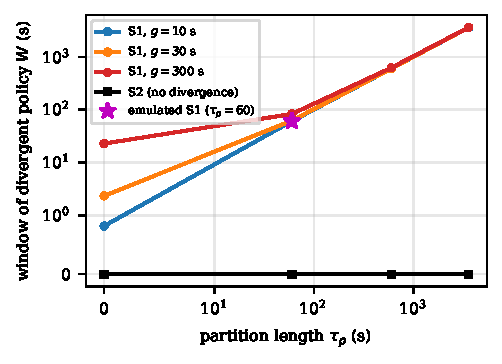
\includegraphics[width=\columnwidth]{fig/fig_window}\caption{E1: divergence window $W$ vs.\ partition length (Monte Carlo) and an emulated protocol run.}\label{fig:window}\end{figure}
The window is set by $\tau_p$, not $g$. Varying the fraction of edges that receive each branch (Fig.~\ref{fig:e1sweep}), S1 diverges on $k(n{-}k)\le36$ pairs and leaves two grants effective on a subset of the fabric; S2 never diverges: the branch held by $\ge T{=}7$ edges commits ($k\le5$: $P'$; $k\ge7$: $P$), at $k{=}6$ the slot stalls until RES, and at most one grant is effective on part of the fabric while the minority catches up.
\begin{figure}[t]\centering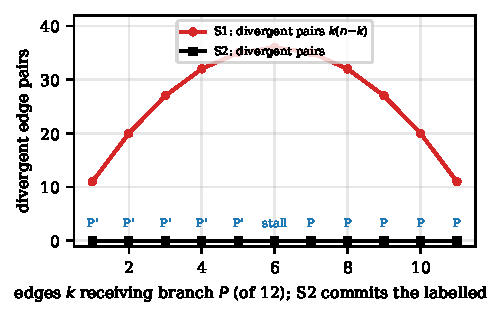
\includegraphics[width=\columnwidth]{fig/fig_e1sweep}\caption{E1 sweep over the split of branches (emulated protocol run, $n{=}12$, $\tau_p{=}60$\,s).}\label{fig:e1sweep}\end{figure}

\textbf{E2, baselines.} S0: edges trust the controller. S1: signed chain with gossip (layer~1 only). S2: Witnessed Policy (layers~1 and~2). S3: BFT-replicated controllers (4 replicas, $f{=}1$, PBFT-style ordering, edges accept on $f{+}1$ matching signed pushes~\cite{morph}), implemented by us for this comparison.
\begin{table}[t]
\centering\caption{Baselines at $n{=}12$, $b{=}1$ (emulated, $\delta{=}50$\,ms).}\label{tab:base}
\scriptsize
\begin{tabular}{@{}p{2.35cm}rrrr@{}}
\toprule
 & S0 & S1 & S2 & S3\\
\midrule
forged entry from a compromised controller: edges accepting & 12 & 0 & 0 & 0 / 12$^\dagger$\\
controller equivocation: divergent pairs & 36 & 36 & 0 & 0\\
commit latency (s) & 0.059 & 0.059 & 0.167 & 0.113\\
messages per slot, $n{=}12$ / $48$ & 12/48 & 12/48 & 300/4656 & 91/243\\
verifications per edge, $n{=}12$ & 1 & 3 & 27 & 4\\
P(commit possible), $a_{ctl}{=}0.999$, $a_{edge}{=}0.9$ & 0.999 & 0.999 & 0.9962$^\ddagger$ & 0.999994\\
\bottomrule
\end{tabular}

\raggedright\scriptsize $^\dagger$ 1 compromised replica / $f{+}1{=}2$ compromised replicas. $^\ddagger$ $a_{ctl}$ times Eq.~\eqref{eq:avail}; stuck slots also need one administrator.
\end{table}
S3 is cheaper than S2 and more available at these parameters; its trust assumption is that fewer than $f{+}1$ controller replicas are compromised. S2 survives compromise of every controller and administrator-approval-free forgery, at $\approx2n^2$ messages per slot and a dependence on edge availability. This is the trade the design makes; if a replicated controller cluster is acceptable, S3 is the cheaper choice.

\textbf{E3, availability.} Eq.~\eqref{eq:avail} is exact for independent edges. Synthetic outage traces (two-state Markov edges, optionally with regional outages; no public SD-WAN outage traces were used) reproduce it for independent edges: over 20 seeds, $0.9973\pm0.0001$ vs.\ $0.9972$ ($T{=}7$) and $0.9108\pm0.0008$ vs.\ $0.9104$ ($T{=}9$) at $a{=}0.9$. Long and regional outages then show what the formula does not cover.
\begin{table}[t]
\centering\caption{E3: $n{=}12$, $b{=}1$; commit possible (mean $\pm$ 95\% CI, 20 seeds) / 99.9th-percentile wait in hours (mean over seeds).}\label{tab:e3}
\scriptsize
\begin{tabular}{@{}lcc@{}}
\toprule
Outage model & separated $T{=}7$ & simple $T{=}9$\\
\midrule
1\,h outages, $a{=}0.90$ & 0.9973$\pm$0.0001 / 0.23 & 0.9108$\pm$0.0008 / 2.5\\
10\,h outages, $a{=}0.90$ & 0.9971$\pm$0.0005 / 2.7 & 0.9109$\pm$0.0035 / 23\\
3 correlated regions + $a{=}0.95$ & 0.9931$\pm$0.0004 / 1.8 & 0.9560$\pm$0.0012 / 11\\
\bottomrule
\end{tabular}
\end{table}
\begin{figure}[t]\centering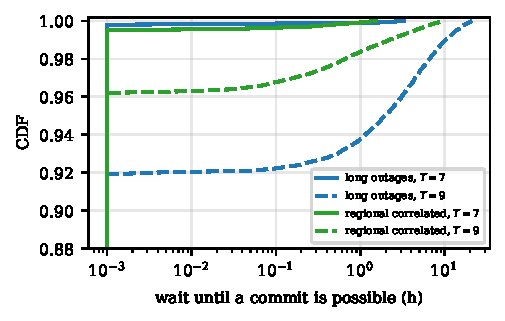
\includegraphics[width=\columnwidth]{fig/fig_e3cdf}\caption{E3: time until a commit is possible, separated vs.\ simple quorum (one run).}\label{fig:e3cdf}\end{figure}

\textbf{E4, incident corpus.} 30 records from nine vendor names (VeloCloud and VMware, Silver Peak and Aruba share product lineages), 2020--2026, each a disclosed vulnerability or incident in an SD-WAN or network management plane (Cisco, Versa, Juniper, Fortinet, Arista VeloCloud, HPE Aruba, Silver Peak, Citrix, VMware). Codebook: capability C1 code execution on the controller (14 records), C4 authentication bypass to administrative control (9), C2 configuration or database write (5), C3 confidentiality only (2). A second coder re-coded all 30 records from the cited sources and agreed on every label ($\kappa{=}1.00$). For nine records this was a source check of a first pass made from the summaries; for the other 21 it was an independent coding. Four records from the 2020 Realmode Labs series rest on a single news article. In 28 of 30 (93\%) exploitation lets the attacker \emph{originate policy} that today's edges accept; all 9 records with exploitation in the wild (e.g., Cisco CVE-2026-20127, FortiManager CVE-2024-47575, Versa CVE-2024-39717~\cite{inc-versa,inc-forti,inc-cisco}) are of this kind. If administrator approval keys are not stored on the controller, layer~1 makes edges reject such policy; it does not address the confidentiality side effects (credential and configuration theft, e.g., FortiManager, Versa, vManage SSH keys) or edge-device compromise. Records are disclosures, not breaches; exploitation is stated for 9 only. The corpus is a search-based sample, not an exhaustive census; later disclosures are not included.

\textbf{E5, prototype.} Python; real Ed25519 signatures and durable attestation records; every edge is an OS process in its own network namespace; the three data-plane edges run WireGuard whose peers and allowed-ips are derived from the \emph{committed} paths and prefixes, plus nftables (default deny, ingress binding, per-grant forward and return rules) rebuilt from the chain. Control messages (TCP) and WireGuard tunnels use separate underlays, so cutting an edge's control network leaves its tunnels up. A probe in the Finance namespace opens real TCP connections to Sales:443 every 0.1\,s through two WireGuard hops. $n{=}7$, $b{=}1$, $T{=}5$ unless stated.
\begin{table}[t]
\centering\caption{Prototype scenarios (real processes, WireGuard, nftables). All rows: 8-vCPU server, kernel WireGuard.}\label{tab:proto}
\scriptsize
\begin{tabular}{@{}p{2.45cm}p{5.3cm}@{}}
\toprule
Scenario & Observed\\
\midrule
grant, then revoke & blocked before; rules installed at all three edges 0.33\,s after the first prepare (edge logs) and all heads committed 0.51\,s after the proposal; the probe sees the first new connection within 0.83\,s (probe timeout 0.7\,s); Guest and Sales:22 blocked; after revoke a new connection is blocked at 0.36\,s and an established session is reset at 0.36\,s; rules removed at all three data-plane edges (Fig.~\ref{fig:rtraffic})\\
endpoint cut off at commit (T9) & committed by quorum; the cut-off endpoint's tunnels are up but it has no rule, so the flow is blocked there; allowed 1.3\,s after its control network returns\\
hub failure (T10) & outage 0.8\,s (3 missed heartbeats), traffic moves to the committed backup tunnel, no chain slot used; switch-back outage 0.1\,s\\
compromised edge (T26, T27) & flow not granted is dropped at the hub's default deny; $0/40$ spoofed packets carrying another site's prefix reach the hub's rules (WireGuard allowed-ips), vs.\ $40/40$ for the edge's own prefix\\
\texttt{kill -9} during install (T18) & ruleset always equals a prefix of the chain (3 rounds, up to 32 grants loaded); after restart it equals the full chain in $4.0$--$4.4$\,s\\
late join (T14, T33) & power-on to ACTIVE $0.5$--$2.5$\,s for $10$--$500$ slots; history $1.27$\,kB per slot ($637$\,kB at $500$); $30$--$60$\,MB RSS\\
equivocation, $n{=}12$ & S1: 36 divergent pairs, fork alert at 20.5\,s ($\tau_p{=}20$\,s); S2: none diverge, RES$\to$commit 0.57\,s, one value, also with a Byzantine process (0.58\,s)\\
$b{=}1$, $c{=}4$ / $c{=}5$ & commits with $7{=}T$ up (0.62\,s) / stalls with 6; commits after heal and re-proposal\\
partition + lease & the cut-off edge removes the rule at 12.8\,s, at its lease expiry (12.5\,s after the partition); the other two edges remove it at 0.5\,s (revocation), which ends end-to-end traffic at 0.33\,s; catches up 0.77\,s after heal (Fig.~\ref{fig:rlease})\\
\bottomrule
\end{tabular}
\end{table}
\begin{figure}[t]\centering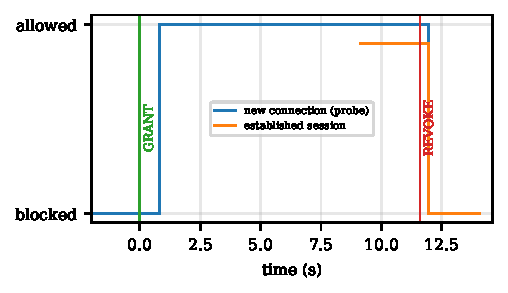
\includegraphics[width=\columnwidth]{fig/fig_real_traffic}\caption{Real packets over WireGuard and nftables: blocked, allowed after commit, then blocked and an established session reset by the revocation.}\label{fig:rtraffic}\end{figure}
\begin{figure}[t]\centering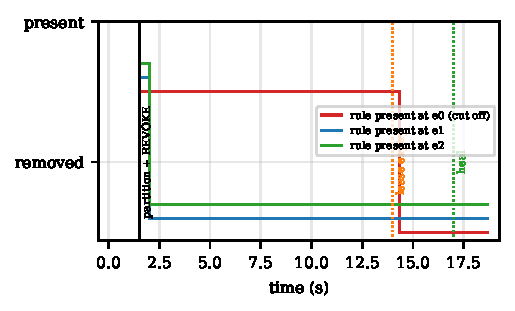
\includegraphics[width=\columnwidth]{fig/fig_real_lease}\caption{Cut-off edge: its rule disappears at lease expiry; the other edges remove it when the revocation commits.}\label{fig:rlease}\end{figure}
\begin{table}[t]
\centering\caption{Cost, one slot, $b=\lfloor(n{-}1)/3\rfloor$. Real processes ($n{\le}32$) and emulator ($n{\ge}100$, $\delta{=}50$\,ms). $^\dagger$Median edge 0.60\,s; messages and verifications at this size exceed the pattern of the other rows, and we have not isolated the cause.}\label{tab:scale}
\scriptsize
\begin{tabular}{@{}rcccc@{}}
\toprule
$n$ & latency S1/S2 (s) & S2 msgs & S2 verif./edge & S2 CPU/edge\\
\midrule
16, server & 0.088 / 0.491 & 512 & 35 & 68\,ms\\
32, server & 0.091 / 2.61$^\dagger$ & 3,072 & 91 & 152\,ms\\
100 & 0.060 / 0.169 & 20,100 & 203 & $\approx$20\,ms\\
200 & 0.060 / 0.169 & 80,200 & 403 & $\approx$39\,ms\\
500 & 0.060 / 0.170 & 500,500 & 1,003 & $\approx$97\,ms\\
\bottomrule
\end{tabular}
\end{table}
Some rules matter in the implementation although the proofs do not state them. An edge calls itself fresh only with heads from $T$ distinct edges, not $b{+}1$. Attestations are retransmitted when an edge returns from an outage, and sync endpoints are pinned so that a wrong endpoint fails closed. The heartbeat timeout follows the measured round-trip time, and the connection probe's timeout scales with the link delay. The transport retries lost messages, and the harness waits until every edge accepts connections before it proposes. Namespace teardown completes before the next topology is built, and a kernel WireGuard device that survives \texttt{kill -9} is reused on restart.

\section{Attacker Capabilities}\label{sec:threat}
\begin{table}[t]
\centering\caption{Outcome by attacker capability (qualitative; rows 1 and 3 are measured in Table~\ref{tab:base}).}\label{tab:threat}
\scriptsize\setlength{\tabcolsep}{3pt}
\begin{tabular}{@{}p{2.2cm}p{1.1cm}p{1.4cm}p{1.5cm}p{1.3cm}@{}}
\toprule
Attacker & S0 & S1 & S2 & S3\\
\midrule
1. controller compromised, no admin keys & any policy & rejected & rejected & rejected$^a$\\
2. plus one key at a tier with $m_\theta{=}1$ & any policy & in-scope grants & in-scope grants & in-scope grants\\
3. controller equivocates (signed fork) & fork & fork until heads cross & no fork & no fork$^a$\\
4. $\ge m_\theta$ admin keys & any policy & any policy & any policy, no fork & any policy, no fork$^a$\\
5. $>b$ edges compromised & those edges & those edges & unique commit not guaranteed & those edges\\
\bottomrule
\end{tabular}

\raggedright\scriptsize $^a$ unless at least $f{+}1$ of the 4 replicas are compromised.
\end{table}
Layer~1 is what stops a single stolen controller credential (row 1), and it already does so with $m_\theta\ge2$ on every tier. Layer~2 adds fork-freedom: it matters when an attacker holds enough approvals to sign two entries (rows 2 and 4) or when a compromised controller equivocates under a partition (row 3), at about $2n^2$ messages per slot and a dependence on edge availability (Table~\ref{tab:base}). The bound $b$ assumes the attacker reaches at most $b$ edges. Edges may share software with each other and with the management plane, so a single vulnerability can compromise several; $b$ should be set to the size of the largest group of edges that share an exploitable component, and software diversity lowers it. With more than $b$ compromised edges unique commit is not guaranteed (row 5).

\section{Related Work}
BFT SDN control planes replicate the controller~\cite{morph,curb}; we witness at the enforcing edges. Signed, threshold-authorized metadata~\cite{tuf,rpki,tailnetlock}, transparency logs and gossip~\cite{ct,gossip} and witness cosigning~\cite{cosi} give tamper evidence; layer~2 adds enforcement-time uniqueness. Configuration verifiers~\cite{batfish,veriflow,minesweeper} check policy offline; here invariants gate commits. Verified distributed systems~\cite{ironfleet,verdi} motivate the TLA$^+$ model. FastPay's lock-once consistent broadcast~\cite{fastpay} is the precedent for the per-round prepare rule; we add round change because an administrator, not a client, must be able to unstick a slot. Flexible BFT~\cite{flexbft} and WHEAT~\cite{wheat} also separate fault classes or reweight quorums; ours separates Byzantine from offline edges for availability. P4BFT~\cite{p4bft} compares replicated-controller outputs in the data plane, closest to S3 here. Minesweeper~\cite{minesweeper} verifies configurations offline. Our quorums are Byzantine quorum systems~\cite{bqs} in the dissemination style, and our one-phase result concerns claim-based recovery at $n=3b+2c+1$; FaB~\cite{fab} commits in one phase with $n\ge5b+1$. Leader-based protocols such as HotStuff~\cite{hotstuff} use $O(n)$ messages where our all-to-all phases use $O(n^2)$. Consistent network updates~\cite{reitblatt} address per-packet consistency during a change and are orthogonal. Reconfiguration of replicated state machines~\cite{lmz} relates to the epochs of Prop.~\ref{prop:epoch}.

\section{Limits}\label{sec:limits}
(i) A stolen $\mathsf{L0}/\mathsf{L1}$ key can create in-scope grants and revoke reachability (denial, not breach). (ii) Genesis is trust-on-first-use, cross-checked out of band. (iii) $b$ must cover compromised edges and lost records (Prop.~\ref{prop:lost}). (iv) Round change needs one available administrator, and an administrator key that signs RES can start ever-higher rounds and delay a stuck slot; requiring $m$ administrator signatures on RES would bound this. (v) TLC models a single slot; epochs are covered by Prop.~\ref{prop:epoch} (proof), the emulated T22 run and the epoch checker. (vi) Props.~\ref{prop:live},~\ref{prop:revoke} are analytic and E1's Monte Carlo models the attack; the data-plane scenarios ran on one 8-vCPU VM (four physical cores), so timings include CPU contention and no multi-host effects; real-process runs reach $n{=}32$, and larger $n$ is emulated. (vii) S3 is our own PBFT-style implementation; outage traces are synthetic; the incident records are disclosures, mostly without stated exploitation, coded by two coders. (viii) Layer~1 assumes administrator approval keys are not stored on the controller. (ix) Freshness takes the $(b{+}1)$-voucher target slot over $T$ heads, so an edge whose heads contain a single honest committer of a revocation can stay fresh without it; Prop.~\ref{prop:revoke} covers connected edges (a) and edges that are not fresh (b), and carrying commit certificates in heads would close the gap. (x) One lease length (about 12.5\,s) is evaluated; the trade-off between lease length and data-plane availability under partition is not.

\section{Conclusion}
Layer~2 gives unique commit with $n\ge3b+2c+1$ edges, claim-based one-phase recovery cannot, and revocation is bounded by $t_c+4\delta+g+d_{\mathrm{enf}}$ (connected) or $\lambda_\gamma+\sigma+d_{\mathrm{enf}}$ (partitioned). The prototype, with real edge processes, WireGuard and nftables, confirms the safety scenarios (the 40 traces and 17 faults of Section~\ref{sec:tlc}) and the cost shape: S2 costs $\approx2n^2$ messages and $\approx3\delta$ per slot, buys immunity to full controller compromise, and a replicated controller (S3) is cheaper when its $f{+}1$ trust assumption is acceptable. A multi-host deployment will test the timing bounds.

\bibliographystyle{IEEEtran}
\bibliography{refs}
\end{document}
